\documentclass[border=10pt]{standalone}

\usepackage{tikz}
\usepackage{tikzsymbols}
\usetikzlibrary{calc,patterns,shapes.geometric}

\def\centerarc[#1](#2)(#3:#4:#5){\draw[#1] ($(#2)+({#5*cos(#3)},{#5*sin(#3)})$) arc (#3:#4:#5);}

\begin{document}
	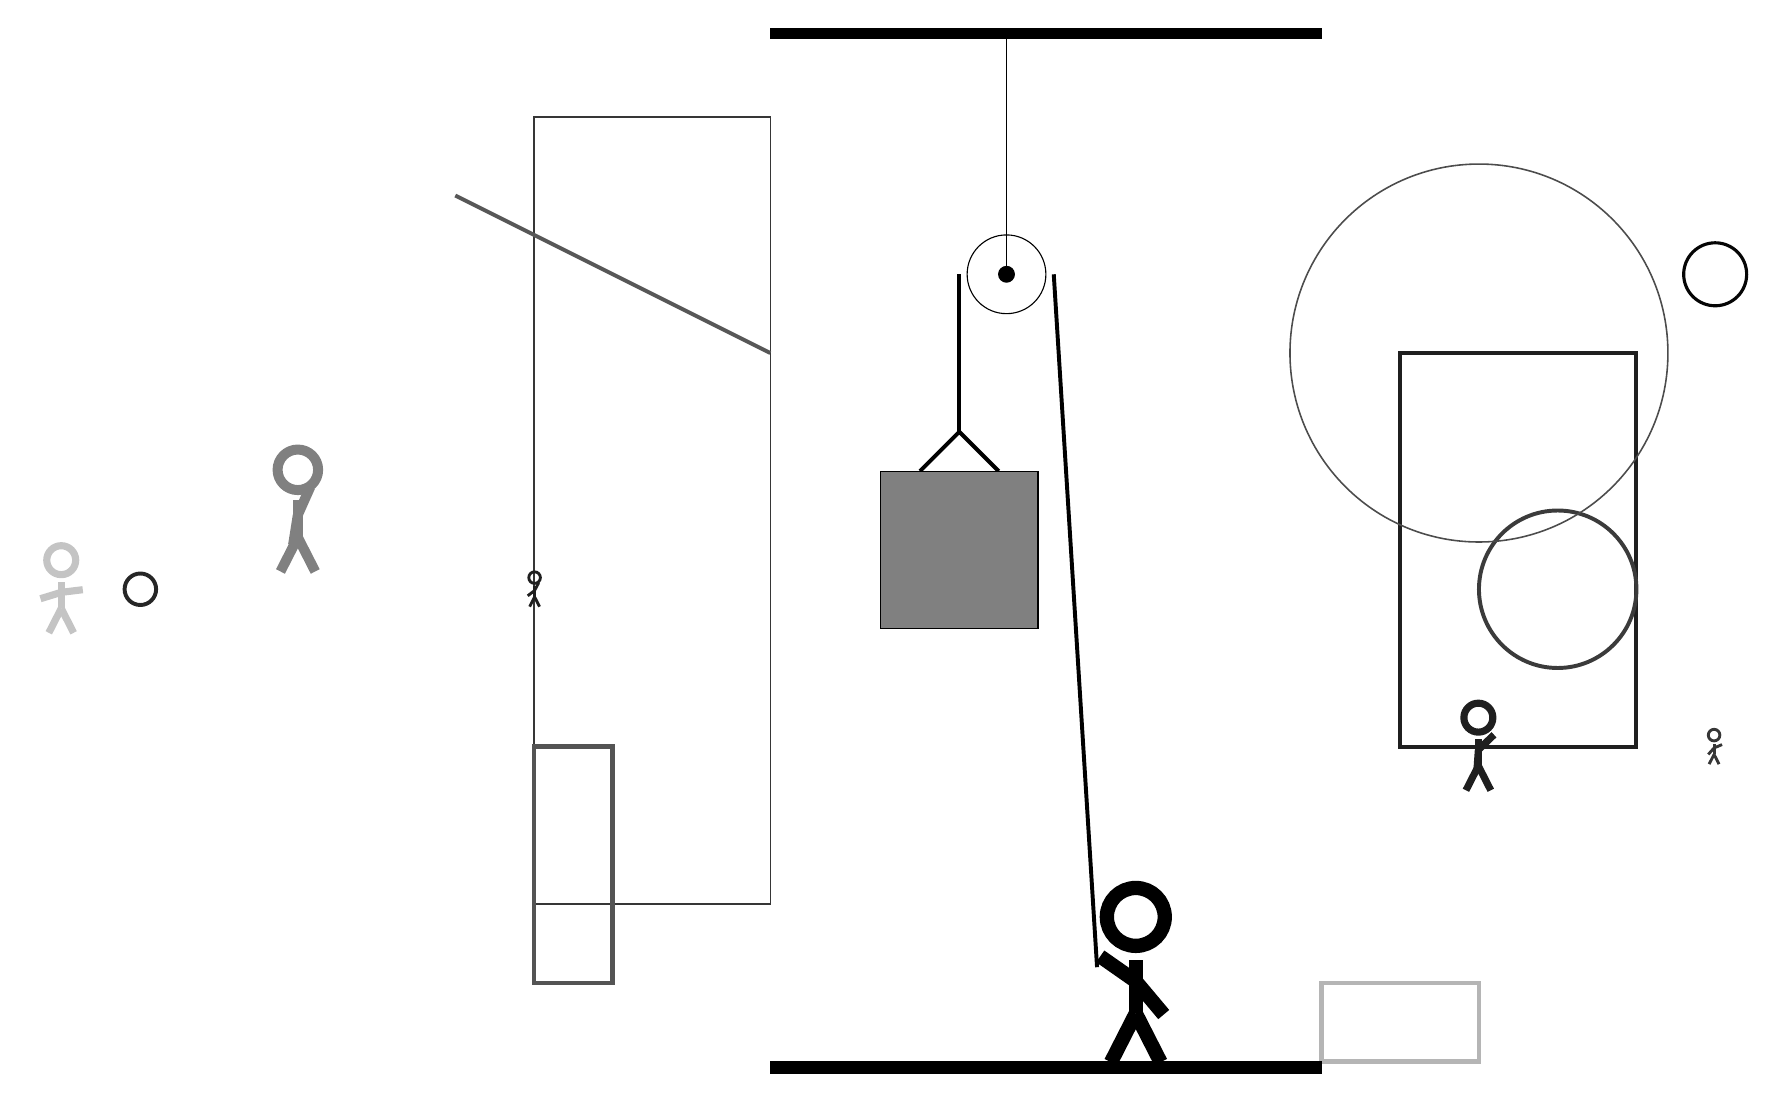
\begin{tikzpicture}
		%%%%% START %%%%%
		
		\draw[fill=black] (-2, 10) rectangle (5, 10.125);
		
		\draw (1, 7) circle (0.5);
		\draw[fill=black] (1, 7) circle (0.1);
		\draw (1, 10) -- (1, 7);
		
		\draw[line width=0.5mm] (-0.1, 4.5) -- (0.4, 5.0) -- (0.9, 4.5);
		\draw[fill=black!50] (-0.6, 4.5) rectangle (1.4, 2.5);
		
		\draw[line width=0.5mm] (0.4, 7) -- (0.4, 5.0);
		\centerarc[line width=0.5mm](1, 7)(0:180:0.6);
		\draw[line width=0.5mm](1.6, 7) -- (2.15, -1.8);
		
		\draw[line width=0.2mm, color=black!79] (-2, 9) rectangle (-5, -1);
		
		\node[line width=0.2mm, color=black!79] at (10, 1) {\Strichmaxerl[2][48][23]};
		\draw[line width=0.5mm, color=black!88] (6, 1) rectangle (9, 6);
		\draw[line width=0.6mm, color=black!29] (5, -3) rectangle (7, -2);
		
		\draw [line width=0.4mm, color=black!98](10, 7) circle (0.4);
		\node[line width=0.2mm, color=black!88] at (7, 1) {\Strichmaxerl[5][86][44]};
		\node[line width=0.6mm, color=black!50] at (-8, 4) {\Strichmaxerl[7][81][66]};
		
		\node[line width=0.7mm, color=black!88] at (-5, 3) {\Strichmaxerl[2][38][62]};
		\draw [line width=0.5mm, color=black!77](8, 3) circle (1.0);
		\draw[line width=0.5mm, color=black!66](-2, 6) -- (-6, 8);
		\draw[line width=0.6mm, color=black!67] (-4, -2) rectangle (-5, 1);
		
		\draw [line width=0.5mm, color=black!85](-10, 3) circle (0.2);
		\draw [line width=0.2mm, color=black!70](7, 6) circle (2.4);
		\node[line width=0.7mm, color=black!23] at (-11, 3) {\Strichmaxerl[5][17][7]};
		
		\node at (2.6, -1.9) {\Strichmaxerl[10][-35][-50]};
		
		\draw[fill=black] (-2, -3) rectangle (5, -3.15);
		
		%%%%% END %%%%%
	\end{tikzpicture}
\end{document}